\section{User Interaction}\label{sec:interaction}
After initializing the flat mesh, we need to refine the model to final state through basic geometric constriant and user-selected constraints which are obtained from user interaction. Our system provides a set of operations to assist users construct the optimized model, such as automatically detecting merging vertexes and symmetric pair on given vertexes, and provide suggestions to allow users click the right option.

%Figure~\ref{fig:interface} illustrates two operations that the system provides, the first one is selecting points need to be merged by users and the second is select the right option from results by vertex merging detection.   

%\begin{figure}
%	\centering
%	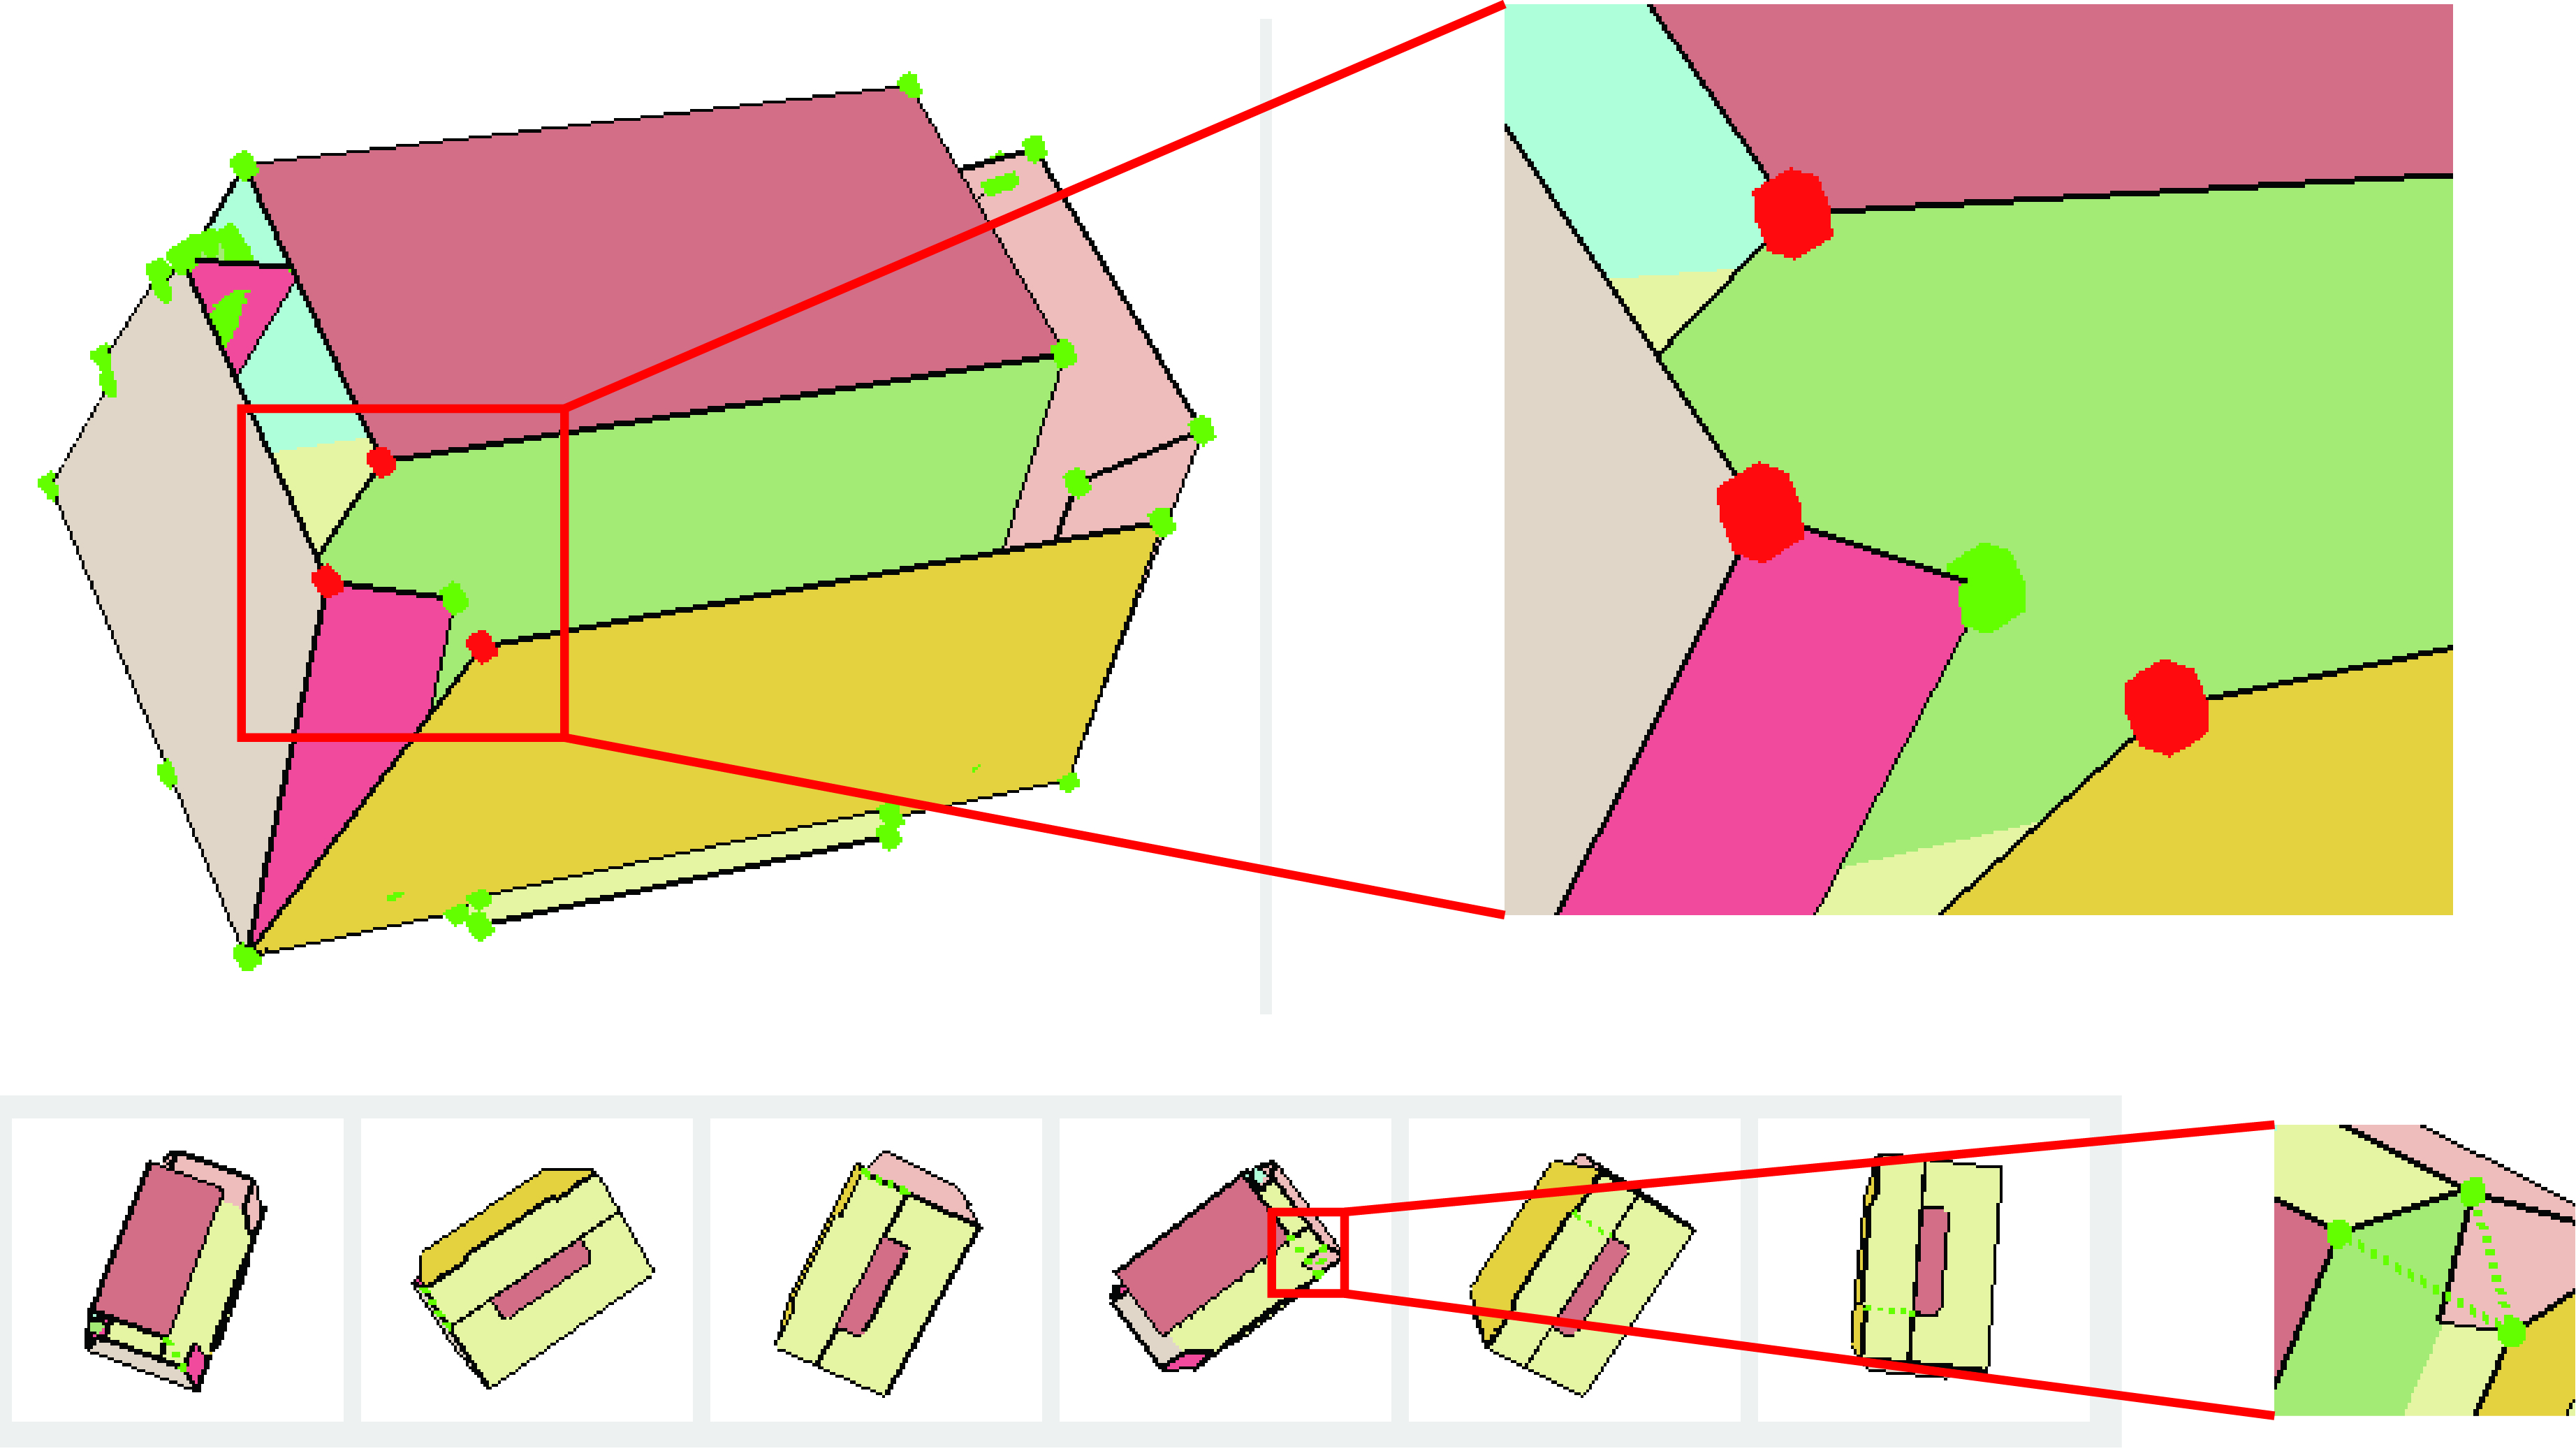
\includegraphics[width=0.9\textwidth]{images/UIdetail.jpg}
%	\caption{two operations that the system provides}
%	\label{fig:interface}
%\end{figure}

\cxj{Explain when modify the 3D model, how to change the 2D layout. }
{\color{blue}{In order to explore more design layouts, our system also allows users edit 3D models by dragging the edges into desired place, and enforce the geometric constraints similar to those described in Sec.~\ref{sec:refinement}. The edge length constraint and face rigidity are still the same, we expanded coplanarity to all the vertexes as they should lie on the same plane. The Irrelevant vertexes which exclude the two vertexes lie on the moving edge stay as close to their original location as well. Figure~\ref{fig:editing} shows one example of 3D editing.}}

\begin{figure}
	\centering
	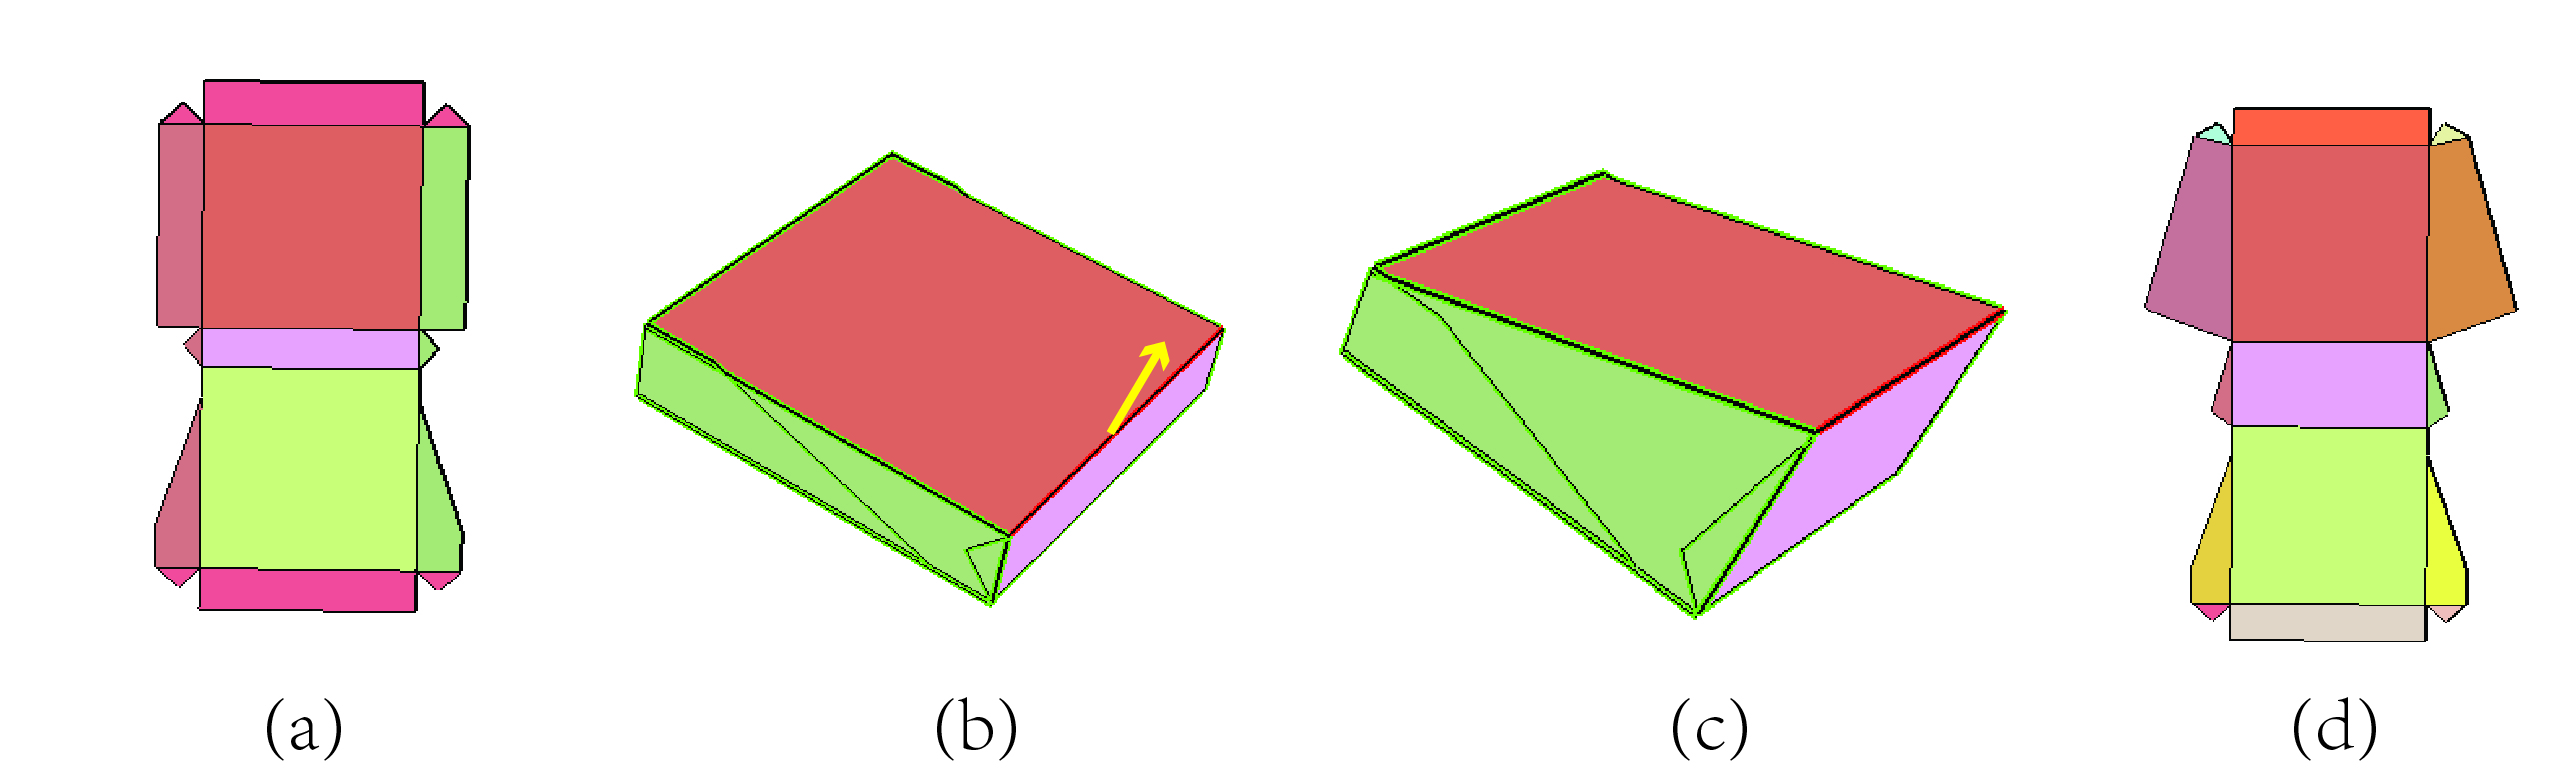
\includegraphics[width=0.7\textwidth]{images/editing}
	\caption{A standard cuboid carton (b) can be generated by the layout (a). Users are allowed to edit the shape of 3D model by dragging the edges, then the model will be deformed to a novel carton (c), by enforce the constrains to layout, our system can generate a deformable layout automatically as (d) shows.}
	\label{fig:editing}
\end{figure}